% Write a piece of TikZ code to show the pedigree diagram of inbreeding between half cousins.
% Use solid circles with gradient fills to display nodes. Display the labels in the diagram where applicable.
% Use any of the required tikz packages to make the code less verbose.

\documentclass{article}
\usepackage{tikz}
\usetikzlibrary{trees,shapes,positioning,arrows.meta,shadows.blur,backgrounds,fit}
\begin{document}

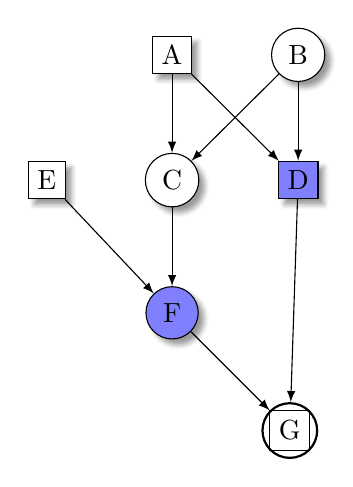
\begin{tikzpicture}[sibling distance=6em,
                    level distance=8em,
                    pF/.style={fill=white, draw, rectangle, text centered, blur shadow},
                    pM/.style={fill=white, draw, circle, text centered, blur shadow},
                    % every node/.style={draw,circle, fill=white, font=\fontsize{10}{10}\selectfont, text centered, blur shadow},
                    ]

% \node (grandfather);
\node[pF] (gpF) {A}; % grandparent female
\node[pM, right=of gpF] (gpM) {B}; % grandparent male
\node[pM, below=of gpF] (father) {C};
\node[pF, below=of gpM,fill=blue!50] (aunt) {D};
\node[pF, left=of father] (mother) {E};
\node[pM, below=of father,fill=blue!50] (nephew) {F};
\draw[thick] node[draw, circle, rotate=0,below right=of nephew] (G){G};
\draw (G.north east) -- (G.south east) -- (G.south west) -- (G.north west) -- cycle;

\draw[-latex] (gpF) -- (aunt);
\draw[-latex] (gpM) -- (aunt);
\draw[-latex] (gpF) -- (father);
\draw[-latex] (gpM) -- (father);
\draw[-latex] (mother) -- (nephew);
\draw[-latex] (father) -- (nephew);
\draw[-latex] (nephew) -- (G);
\draw[-latex] (aunt) -- (G);

\end{tikzpicture}

\end{document}